\documentclass[11pt]{article}

\usepackage{amsmath}
\usepackage{algorithm}
\usepackage{algorithmic}
\usepackage{graphicx}
\usepackage{array}
\usepackage{geometry}
\geometry{margin=1in}
\usepackage{graphicx} 
\usepackage{hyperref}

\title{\textbf{Fake News Detection and Program Optimization
}}
\author{
\begin{tabular}{ccc}
Haitong Lin & Joy Fan & Qing Wen \\
\texttt{hl3266} & \texttt{jf3511} & \texttt{qw919}
\end{tabular}
\\[1.5em]
\begin{tabular}{cc}
Qingyi Cao & Shuling Chen \\
\texttt{qc673} & \texttt{sc10668}
\end{tabular}
}

\date{}

\begin{document}

\maketitle

\section{Introduction}


Fake news detection is an increasingly critical challenge in today's digital age, driven by the rapid dissemination of misinformation online. The proliferation of fake news can lead to significant societal issues, including public confusion, polarization, and erosion of trust in media. Given the vast scale and speed at which information spreads, automated methods for accurately identifying fake news are essential.

In this project, we explore machine learning approaches to effectively distinguish between real and fake news articles. Using the "Fake and Real News Dataset" from Kaggle, we analyze text data and implement classification models to assess accuracy in identifying misinformation. Our approach begins by establishing a baseline using traditional machine learning techniques, specifically logistic regression combined with TF-IDF vectorization.

Subsequently, we optimize the preprocessing and modeling pipeline by applying advanced performance tuning techniques, including Python optimization strategies, Cython compilation, and parallel processing with multiprocessing. Our goal is not only to maintain high model accuracy but also to significantly reduce computational runtime. This paper presents our methodology, optimization strategies, and the comparative results, highlighting effective ways to enhance efficiency in data science workflows while maintaining reliable performance.


\section{Dataset}
We used the “Fake and Real News Dataset” from Kaggle\footnote{\url{https://www.kaggle.com/datasets/clmentbisaillon/fake-and-real-news-dataset/data}}. It contains two CSV files: one for real news articles (sourced from Reuters\footnote{\url{https://www.reuters.com/}}) and one for fake news. The dataset includes a total of 44,919 articles, in which 23,502 are labeled as fake and 21,417 are labeled as real. Each record contains the article’s title, full text, subject category, and publication date. The primary input for our model is the concatenation of the title and text fields. The output is a binary label: 1 for real and 0 for fake news.

The dataset shows clear topical and stylistic differences between the two classes. As shown in Figure~\ref{fig:data}, real news articles tend to be longer and are more likely to cover formal topics such as U.S. politics and global affairs. In contrast, fake news articles are generally shorter and often center on emotionally charged or sensational subjects. Word cloud visualizations reveal that fake articles frequently use vague terms like “said,” “one,” and “people,” while real articles feature more concrete entities such as “trump,” “white house,” and “united states.”

\begin{figure}[H]
    \centering
    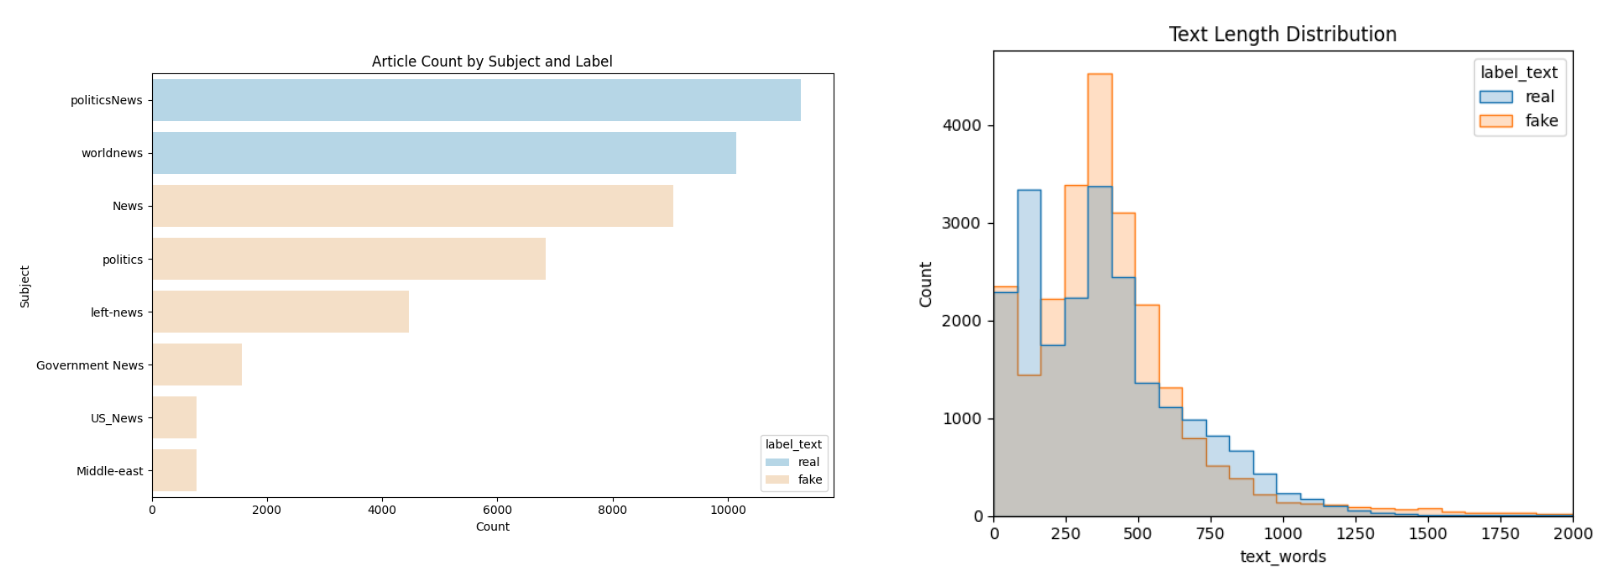
\includegraphics[width=0.9\linewidth]{length.png}
    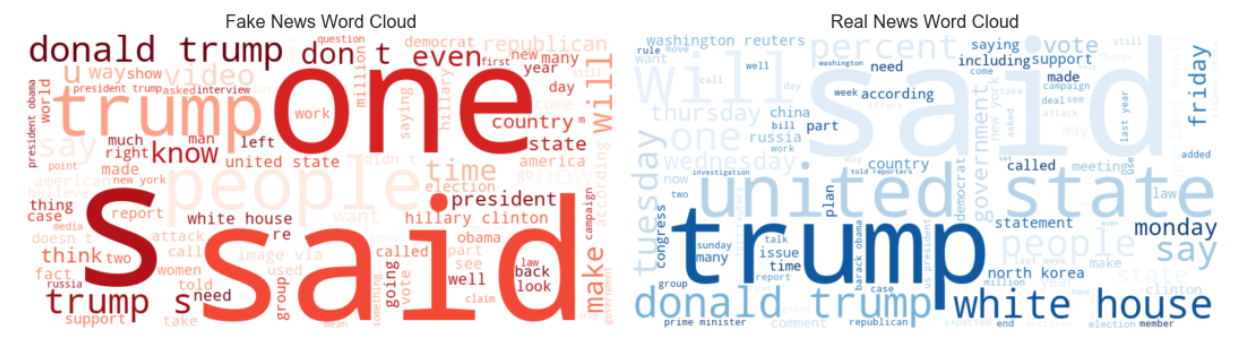
\includegraphics[width=0.9\linewidth]{wordcloud.png}
    \caption{Exploratory Visualizations}
    \label{fig:data}
\end{figure}

\section{Baseline Model}
We developed a baseline model for fake news detection using traditional machine learning techniques. The primary objective was to establish a reference point for evaluating more optimized models in subsequent stages of the project. The dataset consisted of two CSV files containing real and fake news articles. For each article, the title and content were concatenated to form the input text, while the output was a binary label indicating whether the article was real or fake.

To prepare the text data for modeling, we first applied standard preprocessing steps: converting all text to lowercase and removing punctuation as well as non-alphabetic characters. The cleaned text was then transformed using a Term Frequency Inverse Document Frequency (TF-IDF) vectorizer configured with a vocabulary size of 50,000 and English stopwords filtering. This process effectively captured the relevance of individual terms within the documents while reducing noise.

The processed features were split into training and testing sets using an 80/20 ratio. A logistic regression model was trained on the training set with the maximum number of iterations set to 2000 to ensure convergence. We then evaluated the model on the test set using accuracy as the primary metric. The classifier achieved a high accuracy of 99.08\%, demonstrating its effectiveness even in this simple form.

Further evaluation with a confusion matrix indicated a balanced and accurate classification performance across both classes, with 4596 true positives and 4301 true negatives, alongside very few false positives (54) and false negatives (29). Precision, recall, and F1-scores were all 0.99 for both fake and real news classes. The entire training and evaluation process completed in approximately 29.62 seconds.

\begin{figure}[h]  
  \centering
  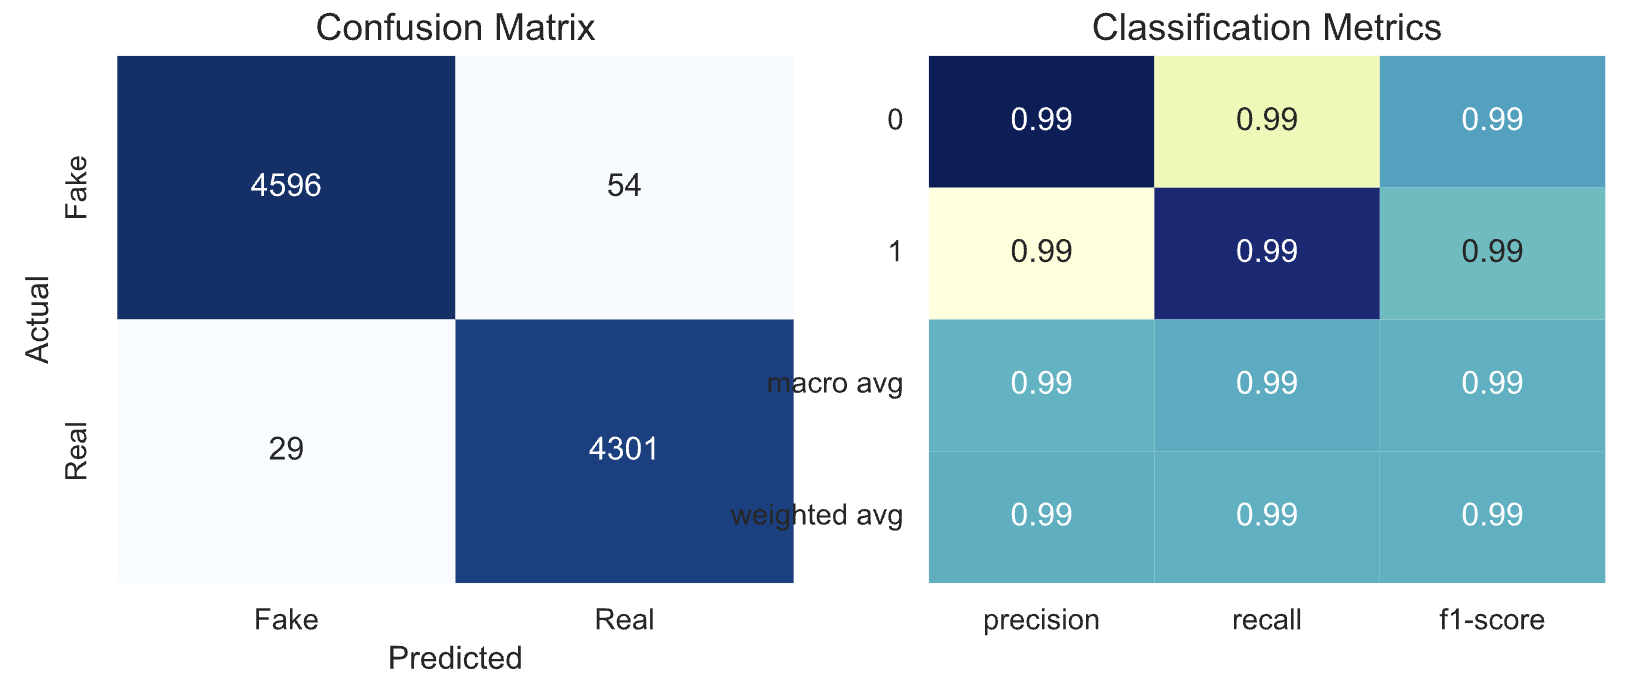
\includegraphics[width=0.9\textwidth]{Confusion Matrix.png} 
  \caption{Confusion Matrix}
  \label{fig:myplot}
\end{figure}

\section{Optimization}
We applied three different optimization methods to improve the runtime performance, while preserving model accuracy at the same time. These methods are directly tied to the performance strategies we discussed in class: Python performance tuning (Lectures 2 and 3), Cython compilation (Lecture 5), and parallel processing with multiprocessing (Lecture 9).

\subsection{Python Performance Tuning: Join.() and Memorization}

The first optimization replaced inefficient string concatenation. In our initial text-cleaning function, we used the \texttt{+=} operator to concatenate characters inside a loop. This approach has time complexity of \textit{O(n\textsuperscript{2})} due to repeatedly copying of intermediate strings. We replaced this with \texttt{"".join(result\_list)}, which achieves time complexity of \textit{O(n)} by building the result incrementally using a list and performing a single join operation at the end.

In addition to that, we implemented memorization to avoid redundant computations. There may be articles sharing identical text. By storing previously cleaned text strings in a cache dictionary, we were able to reuse results instead of re-processing the same input again.

\subsection{Cython Optimization}

To further accelerate the text-cleaning process, we reimplemented the cleaning function using Cython, which allows Python to generate pure C code. We defined a \texttt{.pyx} file containing the cleaning logic and added static types using \texttt{cdef} for variables such as loop indices, individual characters, and intermediate results. This removed Python’s expensive dynamic type checking. This makes a big difference when the loop runs thousands of times. This optimization provided speed improvements with minimal changes to the function’s logic.

\subsection{Cython + Multiprocessing}

Finally, we combined Cython with Python's \texttt{multiprocessing} to parallelize the preprocessing step across available CPU cores. Since each article's text can be cleaned independently, we used \texttt{multiprocessing.Pool} to distribute the text-cleaning work. This step allowed the machine to process multiple articles simultaneously. By combining Cython’s fast execution with parallel workload distribution, this approach resulted in the most significant total time reduction.



\section{Results}
After applying each optimization method, we evaluated the impact in terms of both accuracy and runtime. As shown in the table, all methods — including the baseline and the optimized versions — achieved nearly identical, very high accuracy, approximately 99.08\%. This indicates that none of the optimizations compromised the model’s predictive performance.

In contrast, the runtime showed notable differences across the methods. The baseline implementation required approximately 29.6 seconds to complete. Applying basic Python performance tuning reduced this to around 21.3 seconds. Using Cython alone yielded a similar runtime, approximately 21.9 seconds. The most significant improvement came from combining Cython with multiprocessing, which brought the runtime down to just 15.5 seconds.

\begin{figure}[h]  
  \centering
  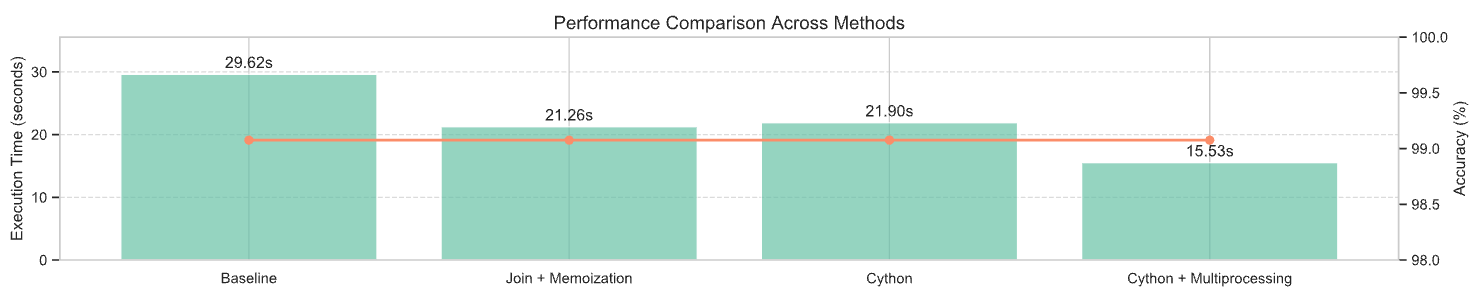
\includegraphics[width=0.9\textwidth]{performance_time.png} 
  \caption{Performance Comparisons Across Methods}
  \label{fig:myplot}
\end{figure}

Looking at the speedup ratios, basic Python tuning achieved a 1.39x improvement over the baseline. Cython alone resulted in a 1.35x speedup. The combination of Cython and multiprocessing delivered the best performance, achieving a 1.91x speedup compared to the original implementation. This method worked best because it leveraged both low-level code optimization and parallel execution, reducing computational overhead and runtime delays.

\begin{figure}[h]  
  \centering
  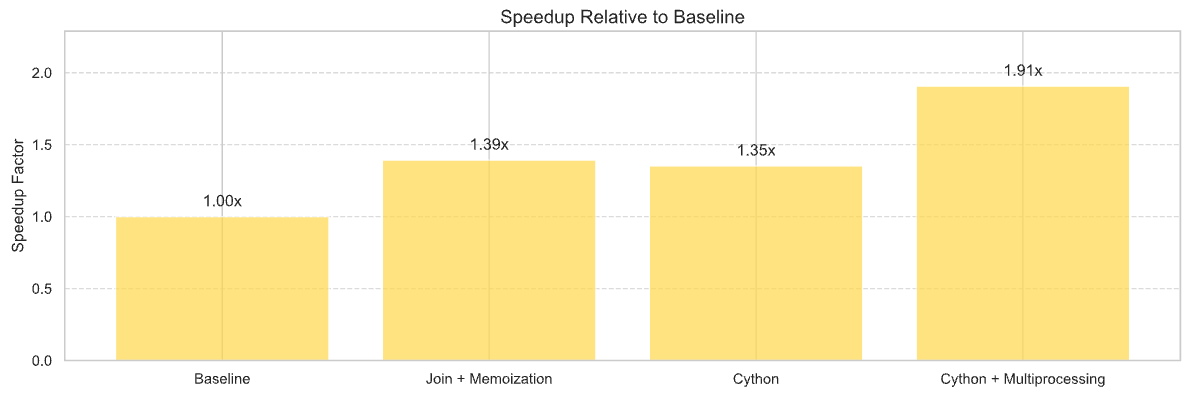
\includegraphics[width=0.9\textwidth]{speedup.png} 
  \caption{Speedup Comparisons}
  \label{fig:myplot}
\end{figure}

While time constraints limited our ability to experiment with additional techniques, future work could explore other optimization strategies or hardware acceleration. Nonetheless, this project offers an interesting exploration of performance tuning and provides a fresh perspective on improving efficiency within the data science pipeline.
\end{document}